Many programs running today use heap object representations that are \emph{fixed}
by the language runtime system.
% , which are not free to vary based on the workload.
For example, the Java and Haskell runtimes dictate an object layout, and the
compiler must stick to it for all programs.
%
In contrast, when humans optimize a program, one of their primary {\em levers on
performance} is changing data representation.  An HPC programmer
knows how to pack a regular tree into a byte array for more efficient
access~\cite{makino90,goldfarb13sc,Meyerovich2011}.

Furthermore, whenever a program receives data from the network or
disk, rigid insistence on a particular heap layout causes an impedance mismatch
we know as {\em deserialization}.
%
%% \note{Compilers normally dictate a standard heap representation for data
%%   manipulated by programs.  Yet substantial performance gains can be had by
%%   operating on data directly in a denser format: the serialization format
%%   already used by incoming data~\cite{}, or a custom format designed by the
%%   programmer, as in HPC applications~\cite{}.}
%
At first glance, the only alternative would seem to be writing low-level code to
deal directly with specialized or serialized data layouts, an error-prone way to
achieve performance optimization at the expense of safety and readability.

In my thesis I propose a way to ameliorate both of these concerns: reify
\emph{data layout} as an explicit part of the program. In short, I am proposing
a \emph{language-based} approach to solving the problem of how to safely program
with serialized data. To that end,
I present a language,
\ourcalc{} (which stands for \emph{location calculus}), whose type system directly
encodes a byte-level layout for algebraic datatypes manipulated by the language.
%
A well-typed program consists of functions, data definitions, \emph{and}
data representation choices, which
% {Well-typed programs are self-describing with respect to their data-layout},
% and that layout
can then be tailored to an application.
%
This means that programs can operate over {\em densely}
encoded (serialized) data in a type-safe way.
%
%% \rn{Somewhat related work: high-level synthesis (hardware) languages that
%%    describe bit-level data using advanced type systems.}

{If data resides on disk in a \ourcalc-compatible format}, it becomes
possible to {\em bring the program to the data} rather than the traditional
approach of bending the data to the code: deserializing it to match the rigid
heap format of the language runtime.
% Its type system ensures that \ourcalc working directly with densely encoded data,
{This effort contrasts with earlier work on persistent
languages~\cite{persistent-java,persistent-objects-thor} and object databases~\cite{object-fault-handling},
which sought to expand the mutable heap to encompass disk as well memory,
translating (swizzling) between persistent pointers and in-memory pointers.  Instead, the
emphasis here is on processing immutable data, and eschewing pointers entirely
wherever possible.}

%% \auditme{Type-safe handling of encoded data applies to \ourcalc programs written by hand,
%% but we also explore synthesizing \ourcalc programs {\em automatically} from
%% vanilla functional programs that say nothing about data layout.}
%% \rn{I think we should perhaps make this less LoCal centric since it is more
%%   HiCal centric once we call it ``Gibbon2''.}

The layout of a \ourcalc{} data constructor by default takes only one (unaligned)
byte in memory and fields may be referred to \emph{either} by pointer
indirections or unboxed into the parent object (serialized). This allows
programmers to interpolate between fully serialized and fully pointer-based
representations.
%
\ourcalc{} can thus serve as a flexible intermediate representation for compilers
or synthesis tools.
% , and I will show how it was used as the intermediate language
% for the Gibbon compiler.

Gibbon is one such compiler. Gibbon is an experimental compiler that
automatically transforms high-level functional programs that operate on
tree-like data into low-level C code that operates directly on serialized data.
Internally, Gibbon represents programs in \ourcalc, so it is able to tune the
memory layout of particular data structures to control precisely how and how
much the data will be serialized. In general, Gibbon produces code that is often
significantly faster than equivalent pointer-based code, with speedups of over
$2\times$ compared to hand-optimized, pointer-based C code, and often much more
than that compared to existing compilers for functional languages like Haskell
and OCaml. In addition to presenting \ourcalc, in this thesis I will cover
the design and implementation of the Gibbon compiler, as well as an evaluation
of the compiler on various benchmarks and applications.

\mav{TODO summarize some applications of Gibbon here}

This thesis will be broken down into three parts. \Cref{chapter:intro} (this
chapter) gives an overview of \ourcalc, with background, motivation, and related
work. \Cref{chapter:local} describes the language and presents a formal
semantics for \ourcalc, as well as some extensions. Finally,
\Cref{chapter:gibbon} presents the Gibbon compiler, which uses \ourcalc{}
internally, and presents an evaluation of Gibbon's performance on various tasks.
A full proof of type safety for the \ourcalc{} language is included in \Cref{appendix:proof}.


%% \section{Background}\label{sec:bg}
% ================================================================================

%% \mav{Many programs batch-process input data from disk or network---parsing
%% logs and reading serialized data formats such as JSON or protobufs.  These
%% programs spend significant time simply \emph{deserializing} data into a
%% memory format that the program can directly work with: for example,
%% pointer-based object graphs in the Java heap. Recently, researchers and
%% industry practitioners have begun to look (again) at unifying internal and
%% external memory representations \cite{cnf-icfp15,capnproto} and}

\section{Motivation}\label{sec:intro-motivation}

\begin{figure}
  \begin{subfigure}[t]{\linewidth}
    \centering
    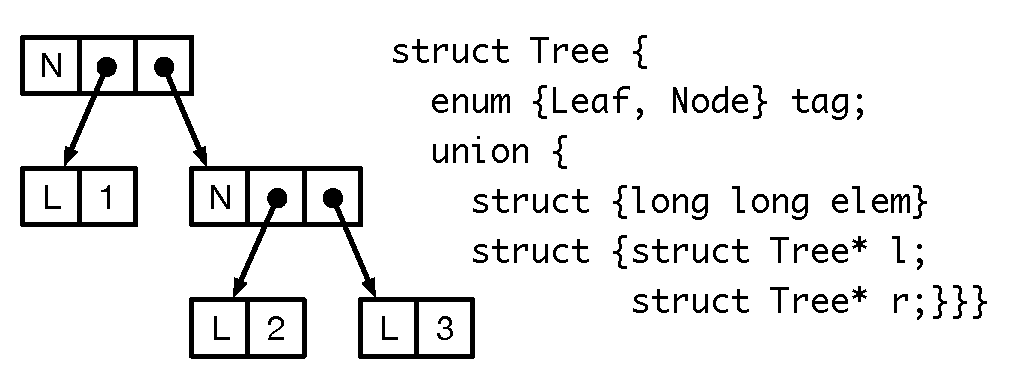
\includegraphics[scale=0.5]{intro-tree-unpacked}
    \caption{Standard representation of a tree structure in C: by default,
      word-sized tags {\em and} pointers.}
    \label{fig:intro-tree-unpacked}
  \end{subfigure}
  \begin{subfigure}[t]{\linewidth}
    \centering
    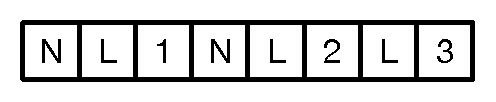
\includegraphics[scale=0.5]{intro-tree-packed}
    \caption{Serialized version of the same tree.  Not to scale: tags take one
      byte and integers eight.}
    \label{fig:intro-tree-packed}
  \end{subfigure}
  \caption{Standard and serialized representations of trees}
  \label{fig:intro-fig}
\end{figure}

Consider the simple tree data structure in \Figref{fig:haskell_tree}, written in
a language that supports algebraic datatypes, where a tree is either a leaf with
an integer or a node with two trees.

\begin{figure}
\begin{subfigure}{\textwidth}
\begin{code}
-- A Tree is either:
--  - a Leaf with an Int, or
--  - a Node with a Tree and a Tree
data Tree = Leaf Int | Node Tree Tree
\end{code}
\caption{Haskell data type representing a binary tree}
\label{fig:haskell_tree}
\end{subfigure}
\begin{subfigure}{\textwidth}
\begin{code}
sum :: Tree -> Int
sum t = case t of
          Leaf n   -> n
          Node x y -> (sum x) + (sum y)
\end{code}
\caption{Function that sums leaf values in a binary tree}
\label{fig:haskell_sumtree}
\end{subfigure}
\begin{subfigure}{\textwidth}
\begin{lstlisting}[language=C++]
int sumPacked (byte * &ptr) {
  int ret = 0;
  if (* ptr == LEAF) {
    ptr++; // skip past leaf tag
    ret = * (int*)ptr; // retrieve integer from leaf
    ptr += sizeof(int); //skip past integer
  } else { // tag must be node
    ptr++; // skip past node tag
    ret += sumPacked(ptr); // sum left sub-tree
    ret += sumPacked(ptr); // sum right sub-tree
  }
  return ret;
}
\end{lstlisting}
\caption{A low-level traversal of serialized tree data written in C++}
\label{fig:cpp-example}
\end{subfigure}

\end{figure}

In memory, each node in this tree is either a \il{Leaf} node, typically
consisting of a header word (denoting that it is a \il{Leaf}) and another word
holding the integer data, or an interior \il{Node}, consisting of a header word
and {\em two} double words (on a 64-bit system) holding pointers to its
children. Depending on the language and runtime system, there is likely additional
space for storing other information about the object, but this is the basic layout.
%
For example, a C
compiler uses 96 bytes
of memory to represent the tree shown in
Figure~\ref{fig:intro-tree-unpacked}.

On the other hand, if we are
sending the tree over the network, we would naturally use a more
compact form in serializing it, as shown in
Figure~\ref{fig:intro-tree-packed}.  In the latter version, we use the
same 24 bytes for the data in the leaves, but only 5 bytes for the
spine (capturing the ``tags'' of the 5 nodes in the tree), rather than
72.  
% A tree with 2 internal nodes and 3 leaf nodes, then, occupies 64 bytes
% of space (20 bytes per internal node and 8 bytes per leaf node), even though it
% contains only 12 bytes of ``useful'' data.
Storing the pointers that maintain
the internal structure of the tree represents a significant storage overhead.


% Though it uses more storage, the usual pointer-based representation is generally easier to manipulate and traverse
% using standard idioms in high-level programming languages.
% % The computation shown in \figref{fig:haskell_sumtree} shows
% % a Haskell function for summing the leaf values in a binary tree, defined by pattern matching and recursion.
% % In comparison, the C++ code for summing a serialized binary tree, shown in
% % \figref{fig:cpp-example}, is less clear, relying on side effects and pointer
% % manipulation.
% But, as mentioned above, even if a programmer was unconcerned with storage
% usage, there would still be situations where the pointer-based representation
% would not be appropriate, such as writing to disk or sending over a network.
% In those situations, the tree
% would be {\em serialized}, with the \il{Node}s and \il{Leaf}s of the tree laid
% out in a buffer in some sequential order. For example, the tree could be
% linearized in a left-to-right preorder, containing {\em tags} to mark data
% constructors and atomic fields such as integers, but ditching the pointers.
% Because it contains no pointers, this serialized representation is
% significantly more compact.
% %
Further, a tree traversal processing this memory representation
follows a precisely linear memory access pattern, because the data is
already laid out in a preorder traversal.
%
On architectures with inexpensive unaligned access, such as modern
x86, this is a desirable in-memory representation as well as a
serialization format.\footnote{Even restricted to aligned access, we
  would still shrink from 72 bytes to 20 by switching to a packed
  format.}
%
But without this structural information, in most settings the
pre-order serialization would be deserialized prior to processing,
requiring more code than the simple \il{sum} function above.

However, this deserialization
is not necessary---it is perfectly possible to write code that performs
the same \il{sum} operation directly on the serialized representation.
All that is necessary is for the code to visit every node in the tree, skipping over
tags and \il{Node} data, and accumulating leaves into the \il{sum}.
%
This traversal can be accomplished in existing languages, writing low-level
buffer-processing code as in the C++ code given in \Figref{fig:cpp-example}.

Essentially, this code operates as follows: \il{ptr} scans along the packed
data structure. For each node type it encounters, it continues scanning
through the node, retrieving the data it needs from the packed representation
(in the case of \il{Leaf}s, the integer, in the case of \il{Node}s,
nothing) and performing the necessary computation. Because this serialized
representation is already in left-to-right preorder, no pointer-like
accesses are necessary: scanning sequentially through the buffer suffices to
access all the nodes of the tree. Note that the \il{sumPacked} function is
still recursive; the program stack helps capture the tree structure of the
data.
%While this isn't strictly necessary for this function, other, more
%complicated traversals may rely on reconstructing the structure.

\begin{figure}
  \begin{subfigure}{\textwidth}
\begin{code}
add1 :: Tree -> Tree
add1 tr =
  case tr of
    Leaf n -> Leaf (n + 1)
    Node a b -> Node (add1 a) (add1 b)
\end{code}
    \caption{add1 in haskell}\label{fig:add1-haskell}
  \end{subfigure}

  \begin{subfigure}{\textwidth}
\begin{lstlisting}[language=C++]
char* add1(char* tin, char* tout) {
  if (*tin == Leaf) {
    *tout = Leaf;
    tin++; tout++;
    *(int*)tout = *(int*)tin + 1;
    return (tin + sizeof(int));
  } else {
    *tout = Node;
    tin++; tout++;
    char* t2 = add1(tin,tout);
    tout += (t2 - t);
    return add1(t2,tout);
  }
}
\end{lstlisting}
    \caption{add1 in c++}\label{fig:add1-cpp}
  \end{subfigure}
\caption{add1 example}
\end{figure}

As another example, consider a function that traverses a binary tree as defined
previously, returns a new binary tree such that each integer has been incremented
by one. This is again straightforward to describe recursively in a language
like Haskell, as shown in \Figref{fig:add1-haskell}.

Like before, we can write a C++ function to do this same computation, only
operating on and returning serialized binary trees. This new function will
have to accept two arguments (pointers to the input and output byte arrays,
respectively), and will additionally return a pointer. The code is shown in
\Figref{fig:add1-cpp}. This time around, the procedure is even more
complicated. Even a single mistake in the pointer arithmetic, such as forgetting
to increment one of the pointers, would lead to a severe error that would
be difficult to debug.


% \begin{comment}
% There are several advantages to working directly on serialized data: the
% serialized representation can take many times fewer bytes to represent than
% a normal pointer-based representation; data can be traversed faster once in
% memory due to predictable memory accesses; \emph{and} data can be read from
% disk without deserialization (e.g. via \texttt{mmap}).
%
%% This motivates contemporary efforts to unify internal and
%% external memory representations like Cap'N Proto~\cite{capnproto}
%% and GHC CNF~\cite{cnf-icfp15}.

Comparing the Haskell procedures operating on traditional trees with the C++
procedures operating on serialized trees, it is clear that working directly with
serialized data is not always easy. First, programs written with typical
pointer-based representations benefit from standard techniques, such as type
checking, to help programmers avoid errors while constructing traversals of
their data structures (so, e.g., type checking can prevent a programmer from
reading an integer value out of an interior node of the tree, or from visiting
the children of a leaf node). But operations on serialized representations
provide no such protection: all of the data in the tree is packed into a flat
buffer that is traversed using cursors. Cursors need to be manipulated carefully
to visit the necessary portions of the buffer---skipping over the sections that
are not needed---and read out the appropriate data, all without the safety net
of a type checker. Hence, writing code to work directly on the serialized data
can be tedious and error-prone.

So, is it possible for programmers to enjoy the benefits of satefy and
convenience that programmers get when using a high-level language, while also
programming directly on serialized data?
%
My proposal is to write the above examples in a language,
\emph{\ourcalc}, that is \emph{expressly designed to use dense serializations}
for its values. The \ourcalc{} \il{sum} function in \Figref{fig:gibbon_sumtree}
extends the simple functional one above with region and location annotations.

\begin{figure}
\begin{code}
sum : forall @\locreg{l}{r}@ . @\tyatlocreg{Tree}{l}{r}@ -> Int
sum [@\locreg{l}{r}@] t = case t of
              Leaf (n : @\tyatlocreg{Int}{l_n}{r}@ ) -> n
              Node (a : @\tyatlocreg{Tree}{l_a}{r}@) (b : @\tyatlocreg{Tree}{l_b}{r}@)
               -> (sum [@\locreg{l_a}{r}@] a) + (sum [@\locreg{l_b}{r}@] b)
\end{code}
\caption{Function that sums the leaf values of a serialized binary tree}
\label{fig:gibbon_sumtree}
\end{figure}

\mav{TODO: include packed add1 gibbon function}

This code operates on serialized data, taking locations of that data (input and
output) as additional function arguments.  It is a {\em region-polymorphic}
function that performs a traversal within region $r$ that contains serialized
data.  Well-typedness ensures that it only reads memory in a type-safe way.
%
Location variables ($\locreg{l}{r}$) have lexical scopes and are introduced as
function arguments and pattern matches.
%
For instance, in the above program, we cannot
access child node locations ($\locreg{l_a}{r}$,$\locreg{l_b}{r}$) until we correctly parse the input
data at $l^r$ and ascertain that represents an intermediate node.
%
Conversely, as I will show later, to \emph{construct} data the type system must
enforce that adjacent fields be serialized consecutively.

I set out to answer the question of whether it is possible to gain the benefits
of programming with serialization without sacrificing safety, and my assertion
is that it is, when using a \emph{language-based approach}. \ourcalc{} is that
language, and the design and implementation of \ourcalc{} is the subject of this
thesis.

\section{Background and Related Work}\label{sec:bg}

My work on \ourcalc{} builds on a lot of existing research on programming languages,
compilers, and systems. In this section I will outline some of this background, and
relate this existing research to the research I am presenting in this thesis.

\paragraph{Serialized data}

Many libraries exist for working with serialized data, and a few
% The library approach is more common, with
% CNF Cap'N Proto
% But compiler-based approaches like Gibbon are not the only option.  There are also
make it easier to use serialized data as in-memory data, or to export the
host-language's pre-existing in-memory format as external data.
% Specifically, we compare our approach to
Cap'N Proto\footnote{An ``insanely fast data interchange format,''
  \url{https://capnproto.org/}, \cite{capnproto}},
is designed to eliminate encoding/decoding by
standardizing on a new binary format for use in memory as well on disk/network.
%% Cap'N Proto allows intra-message pointers, represented as 30-bit relative offsets, but
%% without cycles, and with a unique parent for each node (trees, not DAGs).
%
% Additionally, we compare against
%
{\em Compact Normal Forms} (CNF)~\cite{cnf-icfp15} is
a feature provided by the Glasgow Haskell Compiler since release 8.2.
%
%% This is a
%% feature reminiscent of Lisp and Self systems which save heap snapshots\footnote{For
%%   instance, you can save the Self ``world'' to a \il{.snap} file (\url{selflanguage.org}).  In the Lisp lineage, Chez
%%   Scheme, before version 9, is an example of a system that could save/restore heap
%%   files (\url{www.scheme.com/csug8}).},
%% %
%% except more targeted.
%
The idea is that any purely functional value, once fully evaluated, can be {\em compacted}
into its own region of the heap
--- capturing a transitive closure of its reachable heap.
%% objects, and turning a value of type \il{T} into a \il{Compact T}.
After compaction, the CNF can be stored externally and loaded
back into the heap later.

Example of Haskell CNF\figref{fig:haskellcnfexample}.

\mav{Include an example and some further explanation of Haskell CNF}

{Persistent languages tackle the problem of automatically moving data between disk
and in-memory representations~\cite{persistent-java,persistent-object-systems,persistent-objects-thor}, and can swizzle pointers as part of this
translation to create more efficient representations. However, like CNF, these
representations still maintain pointers, so cannot realize the full advantage of
our system.}

\paragraph{Tracking resource usage in types}

\mv{Include some references for ordered types and linear types, as well as region types.
  There's a lot of related work there to talk about with respect to the techniques going
  into the type system, even if they're not really related to the overall goal of programming
  with serialiezd data.
}

For decades there has been significant research into using types to track and
constrain resource use in programming languages. In the 1980s, researchers like
Lucassen and Gifford developed effect type systems~\cite{effect-types} which use
types to perform side-effect analysis. Their approach involves a type system
with three \emph{kinds}: types, which describe the value that an expression may
evaluate to; effects, which describe the side-effects that an expression may
perform; and regions, which describe the area of the store in which side-effects
may occur.

Effect systems~\cite{effect-types}, Cyclone~\cite{cyclone-pldi}, Region
calculi~\cite{mlkit-retrospective}.

Another commonly discussed way to manage resources, and particularly memory,
using types in functional programs is the use of \emph{linear
types}~\cite{wadler-linear-types}. Values that have a linear type must be used
exactly once, and (as Wadler writes), just like the world, they can not be
duplicated or destroyed. Because of this, they do not require garbage
collection, so a functional programmer may use linear types to construct
programs that need no automatic memory management. Additionally, linear types
can be used to do in-place updates to mutable data structures in a functional
way. This second property is important to this thesis, as later, in
\secref{subsec:linear}, I show how this property of linear types can be used to
safely write and read serialized data in Linear Haskell (an extension so the Haskell
programming language that adds support for linear types).


\paragraph{Compiler support for external dense data}

If we look instead at compiler support for computing with data in dense or
external forms, there are many compilers for stream processing
languages~\cite{streamit,wavescript-nsdi}---or restricted languages such as
XPath~\cite{xpath-streams}---that generate efficient computations over data
streams.

Overview of XPath.

Overview of StreamIt.

These are somewhat related, but \ourcalc differs in targeting general
purpose recursive functions over algebraic datatypes.


\mav{Include brief overview of XPath and Stream-It/WaveScript.}

%
%% In this category, the main published approach is our prior work on Gibbon~\cite{ecoop17-gibbon},
%% which compiles idiomatic programs to operate
%% on serialized data.  However, the Gibbon approach described previously can only handle fully
%% serialized data and thus introduces asymptotic slowdowns as we'll see in the
%% next section.  (At the time, we considered adding indirections as future work but
%% they were not part of the compiler.)
%% %
%% Also, the prior Gibbon compiler had no analogue to our location calculus: no way for a
%% type-system to enforce correct handling of regions and locations within
%% serialized data---which provides a much stronger foundation for building such compilers.

\paragraph{Fusion and deforestation}

\emph{Deforestation} is the technique of removing intermediary list/tree-like
data in functional computations~\cite{wadler-deforestation}.
%
For example (taken from Wadler's original paper), given the functional program
\il{sum(map square (upto 1 n))}, a compiler or interpreter would generally have
\il{upto 1 n} return a list of numbers from $1$ to $n$, then have the \il{map}
procedure return a new list with the numbers squared, and finally have \il{sum}
consume this list and return an integer. This style of programming is convenient,
because it allows programmers to build their programs out of general, re-usable
procedures like \il{map} and \il{upto}, but it results in unnecessary memory
allocation in the form of intermediary structures. Deforestation transforms
this computation and removes the need to allocate intermediary lists, instead
computing the sum directly via a single tail-recursive procedure.

The problem of computing \emph{without} deserializing can be viewed as a
fusion/deforestation problem: to fuse the compute loop with the deserialize
loop. But traditional deforestation approaches like
Wadler's~\cite{wadler-deforestation}, don't rise to being able to handle a full
deserializer, and popular approaches based on more restrictive \emph{combinator
libraries}~\cite{stream-fusion} are less expressive than \lamadt{} and
\ourcalc{}.

Example of Wadler's treeless language \figref{fig:treeless}.

\paragraph{Ornaments}

\emph{Ornaments} are a body of theory regarding connections between related
data structure that differ based on additions or
reorganization~\cite{ornaments}.
%
Indeed, \ourcalc's addition of offset fields to data {\em is} ornamentation.
%
Practical implementations of ornaments~\cite{ornament-ml} provide support for
lifting functions across types related by ornaments, transforming the code.
%
However, the isomorphism between a datatype and its serialized form is not an
ornament, and thus lifting functions across that isomorphism is not supported.

%% \ourcalc does not allow construction of cyclic values (only DAGs), so it is less
%% related to graph-processing systems.

\paragraph{Compiler optimizations for tree traversals}

\ourcalc relates to a broader literature on optimizing
tree-traversing programs and heap representations.
%
There has been significant work in optimizing the layout and
traversal patterns of tree data structures for performance reasons.
%
The most closely related line of work is \emph{cache-conscious structure
  layout}~\cite{chilimbi1999}, which proposes a data layout scheme that lays out
the nodes of a tree according to an order determined by a provided traversal
function. Because this layout is determined by a specific traversal function,
it serves a similar purpose to the linearization of data in our packed layout:
when trees are traversed in the same manner as the layout order, spatial
locality is improved. Note, however, that Chilimbi et al.'s approach does not
change the internal structure of objects, nor the code that traverses those
data structures. Hence, all pointers are preserved, and this approach does not
offer the additional benefits of our packed layout such as denser accesses and
avoidance of pointer indirection. Other spatial locality
work~\cite{Truong1998,Lattner2005,Chilimbi1999a} has similar effects and
limitations to cache-conscious structure layout.

One exception is Chilimbi et al.'s work on {\em automatic structure
splitting}~\cite{Chilimbi1999b}, where objects are transformed into split
representations, allowing hot fields from multiple objects to be co-located on
a single cache line while those objects' cold fields are placed elsewhere.
Because this layout optimization changes the internal representation of the
object, Chilimbi et al. develop a compiler pass that automatically transforms
code to work with the split representation. The transformations for structure
splitting concern how to access object fields, and hence, unlike our work, do
not require deeper transformations to remove the pointer dereferences inherent
in traversing linked data structures. Indeed, neither this work nor
cache-conscious structure placement affect the behavior of pointers in data
structures.

\emph{Automatic pool allocation}~\cite{Lattner2005} proposes
allocating disjoint data structures into disjoint partitions of
memory, and this approach can be extended with compression
optimization~\cite{Lattner2005mspc}. Because a data structure is
allocated into an isolated pool, ``internal'' pointers that connect
nodes of that data structure definitely do not access arbitrary memory
locations, and hence can use narrower bit widths to save space. Unlike
the spatial locality work discusses in the previous paragraph, this
compression optimization both shrinks the overall representation of
the data structure (as in our packed representation) and utilizes
compiler rewrites to do so (as in our compiler transformations).

% Tree linearization, and the attendant changes required to traversal code, are
% common in high-performance computing settings, especially for
% vectorization~\cite{makino90,goldfarb13sc,Meyerovich2011,ren13cgo,ren14taco}.
% These approaches, by closely matching data structure layout to the traversal
% behavior of specific applications, can eliminate many pointer dereferences,
% compress data structures, and simplify traversal implementations. However, all
% of these approaches are programmer-directed: either \emph{ad hoc},
% application-specific
% implementations~\cite{makino90,goldfarb13sc,Meyerovich2011}, or driven by
% library functions that the programmer must exploit~\cite{ren13cgo,ren14taco}.

\paragraph{Array-based approaches to traversing tree-like data}

Hsu looks at a representation of abstract syntax trees that uses a matrix
layout, allowing operations to be specified in a data-parallel manner without
traversing pointers~\cite{hsu2016key}. While this representation shares a goal
with ours of avoiding pointers, it is not ``packed''---the representation
requires a dense representation of a sparse matrix---and hence does not yield
the type of space savings we target.

In the high-performance computing community, linearizing trees and tree traversals for improved
performance has been a common technique~\cite{makino90,goldfarb13sc}. These
linearizations tend to be {\em ad hoc}, written specifically for a given
application, and each application must be re-written by hand to benefit. This
contrasts with our compiler-based approach which allows programmers to write
using idiomatic traversal algorithms, relying on the compiler to synthesize
the packed representation as well as the algorithm to traverse that
representation.

Similar {\em ad hoc} layout transformations have recently been pursued in the
context of vectorization~\cite{Meyerovich2011,ren13cgo,ren14taco}. Meyerovich
et al. discuss different linearization schemes that can promote packed SIMD
loads and stores, improving vectorization efficiency~\cite{Meyerovich2011}.
These layouts have the implicit effect of eliminating pointer dereferences, as
in our packed representations, but rely on index arithmetic to traverse
formerly-linked nodes, rather than encoding particular traversal orders. Ren
et al. look at a wide range of tree layouts for vectorization, each targeted
at different traversal patterns~\cite{ren13cgo,ren14taco}. These layouts are
chosen to match the traversal patterns of an application, enabling the removal
of pointers, as in our layouts. Ren et al. use a library-based approach:
applications are written using high-level tree interfaces, with specific
layouts chosen based on hardware and application considerations. In contrast,
this work focuses on compiler-driven transformations of both the tree layout
and the code that traverses the tree.

Nested data parallelism~\cite{nested-data-parallel}.
Array programming~\cite{array-programming}.
\mav{Have a few paragraphs on general array programming and on flattening
  and nested data parallelism.}
